% ============================================================
%  Tutorial: Diffusion Models → Discrete DLMs → Privacy → MIA
%  Compile:  pdflatex (×2)  →  bibtex  →  pdflatex (×2)
% ============================================================
\documentclass[10pt, aspectratio=169]{beamer}

\usetheme[progressbar=frametitle]{metropolis}
\usepackage{appendixnumberbeamer}
\usepackage{booktabs}
\usepackage{amsmath,amssymb,mathtools}
\usepackage{graphicx}
\usepackage{xcolor}
\usepackage{multirow}
\usepackage{array}
\usepackage{algorithm}
\usepackage{algpseudocode}
\usepackage[round]{natbib}

\graphicspath{{/Users/skumar/Desktop/DA5001/Project/Project/Midterm_Report/plots_ppt/}}

\setbeamercolor{progress bar}{fg=orange!80!black, bg=orange!25!white}
\metroset{block=fill}

\DeclareMathOperator*{\E}{\mathbb{E}}
\newcommand{\MASK}{\texttt{[MASK]}}
\newcommand{\bx}{\mathbf{x}}
\newcommand{\NLL}{\mathrm{NLL}}
\newcommand{\KL}{D_{\mathrm{KL}}}

\title{Diffusion Models, Discrete DLMs,\\and Membership Inference: A Tutorial}
\author{Shailesh K}
\institute{Indian Institute of Technology Madras \\ DA5001: Privacy in AI}
\date{}

% ===========================================================================
\begin{document}
% ===========================================================================

\maketitle

\begin{frame}{Roadmap}
  \begin{columns}[T]
    \column{0.48\textwidth}
    \textbf{Part I: Continuous Diffusion}\\[3pt]
    \quad Generative models \& motivation\\
    \quad Forward process (full derivation)\\
    \quad Reverse process\\
    \quad ELBO, step-by-step derivation\\[8pt]
    \textbf{Part II: From Images to Text}\\[3pt]
    \quad How LLMs work\\
    \quad Discrete diffusion (D3PM + MDLM)\\
    \quad AR vs DLM comparison
    \column{0.48\textwidth}
    \textbf{Part III: Privacy Foundations}\\[3pt]
    \quad $(\varepsilon,\delta)$-DP, attacker-defender\\
    \quad Membership inference\\[8pt]
    \textbf{Part IV: MIA Research Survey}\\[3pt]
    \quad 6 key papers (method / algorithm / results)\\[8pt]
    \textbf{Part V: SAMA and Our Work}\\[3pt]
    \quad SAMA attack\\
    \quad DT-MIA features \& results
  \end{columns}
\end{frame}

% ===========================================================================
\section{Part I: Continuous Diffusion Models}
% ===========================================================================

% ── Generative models: deep dive ────────────────────────────────────────────

\begin{frame}{The Generative Modelling Problem}
  \textbf{Goal:} given a dataset $\{x^{(i)}\}_{i=1}^N$, learn the true distribution $p_{\mathrm{data}}(x)$
  so we can draw new, realistic samples.\\[10pt]
  This looks simple, but the data lives on a high-dimensional manifold ($\sim$millions of dimensions for images/text).
  Direct density estimation is hopeless.\\[10pt]
  Four families of models have been developed, each with a different strategy.
\end{frame}

\begin{frame}{Variational Autoencoders (VAEs)}
  \textbf{Idea:} compress data into a low-dimensional latent code $z$, then reconstruct.
  \[
    p_\theta(x) = \int p_\theta(x \mid z)\,p(z)\,dz
  \]
  \begin{itemize}
    \item Encoder $q_\phi(z\mid x)$ maps data to a Gaussian in latent space
    \item Decoder $p_\theta(x\mid z)$ maps back to data space
    \item Trained by maximizing the ELBO (a lower bound on $\log p(x)$)
  \end{itemize}
  \textbf{Problem:} the Gaussian bottleneck forces the decoder to average over many plausible outputs.
  Generated samples are often blurry and lack fine detail.
\end{frame}

\begin{frame}{Generative Adversarial Networks (GANs)}
  \textbf{Idea:} train a generator $G$ and discriminator $D$ against each other.
  \[
    \min_G \max_D \;\E[\log D(x)] + \E[\log(1 - D(G(z)))]
  \]
  \begin{itemize}
    \item Generator maps noise $z \sim \mathcal{N}(0,I)$ to realistic samples
    \item Discriminator learns to distinguish real from generated
    \item No explicit density, generation is a single forward pass
  \end{itemize}
  \textbf{Problems:}
  \begin{itemize}
    \item \textbf{Mode collapse:} generator memorizes a few good outputs, ignores the rest
    \item \textbf{Training instability:} the min-max game is notoriously hard to balance
    \item No exact likelihood; cannot easily evaluate $p(x)$
  \end{itemize}
\end{frame}

\begin{frame}{Normalizing Flows}
  \textbf{Idea:} learn an invertible transformation $f$ from data space to a simple prior.
  \[
    p_\theta(x) = p(f(x))\,\left|\det \frac{\partial f}{\partial x}\right|
  \]
  \begin{itemize}
    \item Exact log-likelihood via the change-of-variables formula
    \item Inference and generation are just $f$ and $f^{-1}$
  \end{itemize}
  \textbf{Problem:}
  \begin{itemize}
    \item $f$ must be \textbf{invertible}, which severely limits architecture design
    \item Computing $\det(\partial f/\partial x)$ requires special structure (triangular Jacobian)
    \item Hard to scale to high-dimensional data; generated samples are lower quality than GANs
  \end{itemize}
\end{frame}

\begin{frame}{Why Diffusion? The Key Insight}
  Diffusion models sidestep all three issues:
  \begin{itemize}
    \item \textbf{No bottleneck} (unlike VAEs), the latent space has the same dimension as the data
    \item \textbf{No adversary} (unlike GANs), training is a simple regression problem, highly stable
    \item \textbf{No invertibility constraint} (unlike flows), the model is a free-form neural network
  \end{itemize}
  \vspace{8pt}
  The trade-off: generation requires \textbf{many forward passes} (iterative denoising).\\[6pt]
  In practice, this is acceptable, diffusion models produce the highest-quality samples known.
\end{frame}

% ── Forward process ─────────────────────────────────────────────────────────

\begin{frame}{Forward Process: The Core Idea}
  Instead of learning how to generate from scratch, we learn how to \textbf{undo noise}.\\[10pt]
  \textbf{The plan:}
  \begin{enumerate}
    \item Define a fixed procedure that gradually destroys any data point into noise
    \item Train a neural network to reverse this destruction, one small step at a time
  \end{enumerate}
  \vspace{10pt}
  \begin{center}
    \large
    $x_0 \;\xrightarrow{+\varepsilon}\; x_1 \;\xrightarrow{+\varepsilon}\; \cdots \;\xrightarrow{+\varepsilon}\; x_T \approx \mathcal{N}(0,I)$
  \end{center}
\end{frame}

\begin{frame}{Forward Process: One Step in Detail}
  At step $t$, we add a \textbf{small} Gaussian perturbation to $x_{t-1}$:
  \[
    q(x_t \mid x_{t-1}) = \mathcal{N}\!\bigl(x_t;\;\sqrt{1-\beta_t}\,x_{t-1},\;\beta_t\,I\bigr)
  \]
  Unpacking this:
  \begin{itemize}
    \item $x_t = \sqrt{1-\beta_t}\,x_{t-1} + \sqrt{\beta_t}\;\varepsilon_t, \quad \varepsilon_t \sim \mathcal{N}(0,I)$
    \item $\sqrt{1-\beta_t}$ \textbf{shrinks} the signal: $\beta_t$ small $\Rightarrow$ mostly preserved
    \item $\sqrt{\beta_t}$ scales the noise added
    \item Since $\beta_t \in (0,1)$, the signal amplitude decays at every step
  \end{itemize}
  \vspace{6pt}
  The signal shrinks and noise accumulates until $x_t$ is indistinguishable from $\mathcal{N}(0,I)$.
\end{frame}

\begin{frame}{Forward Process: How It Becomes Pure Gaussian Noise}
  After $t$ steps the signal has been scaled by $\prod_{s=1}^t \sqrt{1-\beta_s}$.
  Each factor is $< 1$, so the product shrinks exponentially:
  \[
    \prod_{s=1}^{T}\sqrt{1-\beta_s} \;\to\; 0 \quad \text{as } T \to \infty
  \]
  Simultaneously, the accumulated noise has variance $\sum_{s=1}^t \beta_s \prod_{k>s}(1-\beta_k)$,
  which approaches $1$.\\[8pt]
  \textbf{Result:} after enough steps, $x_T \approx \mathcal{N}(0,I)$, regardless of what $x_0$ was.
  The original data has been completely destroyed.\\[6pt]
  This gives us a clean known starting point for generation: just sample from $\mathcal{N}(0,I)$.
\end{frame}

\begin{frame}{Forward Process: Tracking the Cumulative Noise}
  Let's define shorthand for the cumulative factors.
  After $t$ steps, how much signal remains?
  \[
    \alpha_t = 1 - \beta_t \quad\text{(signal retained at step }t\text{)},\qquad
    \bar\alpha_t = \prod_{s=1}^{t}\alpha_s \quad\text{(total signal retained after }t\text{ steps)}
  \]
  \begin{itemize}
    \item $\bar\alpha_t$ starts near $1.0$ and decays toward $0$
    \item At step $t$: signal has amplitude $\sqrt{\bar\alpha_t}$, noise variance is $1 - \bar\alpha_t$
    \item This directly tells us how much of $x_0$ survives to $x_t$
  \end{itemize}
\end{frame}

\begin{frame}{Forward Process: The Marginal: Skipping the Chain}
  We don't need to iterate all $t$ steps.
  Because each step is Gaussian, the product of Gaussians is Gaussian, and the whole chain collapses:
  \[
    \boxed{q(x_t \mid x_0) = \mathcal{N}\!\bigl(x_t;\;\sqrt{\bar\alpha_t}\,x_0,\;(1-\bar\alpha_t)\,I\bigr)}
  \]
  Equivalently, sample $x_t$ at any noise level in one shot:
  \[
    x_t = \underbrace{\sqrt{\bar\alpha_t}\,x_0}_{\text{signal, scaled by }\sqrt{\bar\alpha_t}}
        + \underbrace{\sqrt{1-\bar\alpha_t}\;\varepsilon}_{\text{noise}}, \qquad \varepsilon \sim \mathcal{N}(0,I)
  \]
  \textbf{Why this matters:} during training, we sample a random $t$
  and corrupt $x_0$ in a single matrix multiply, no sequential simulation needed.
\end{frame}

% ── Reverse process ─────────────────────────────────────────────────────────

\begin{frame}{Reverse Process: What We Want to Learn}
  The forward process destroys data in a known, tractable way.
  The model must learn to invert it:
  \[
    p_\theta(x_{t-1} \mid x_t) \approx q(x_{t-1} \mid x_t)
  \]
  \textbf{Why can't we just invert $q$ directly?}\\
  \begin{itemize}
    \item $q(x_{t-1}\mid x_t) = \int q(x_{t-1}\mid x_t,x_0)\,q(x_0\mid x_t)\,dx_0$, requires knowing $p(x_0)$, which is what we're trying to learn
    \item However: when $\beta_t$ is small, the reverse step is \textbf{also} approximately Gaussian
    \item So we parameterize $p_\theta(x_{t-1}\mid x_t)$ as a Gaussian with a learned mean
  \end{itemize}
\end{frame}

\begin{frame}{Reverse Process: Gaussian Parameterization}
  We model the reverse step as:
  \[
    p_\theta(x_{t-1} \mid x_t) = \mathcal{N}\!\bigl(x_{t-1};\;\mu_\theta(x_t,t),\;\sigma_t^2\,I\bigr)
  \]
  \begin{itemize}
    \item Variance $\sigma_t^2 = \beta_t$ or $\tilde\beta_t = \frac{1-\bar\alpha_{t-1}}{1-\bar\alpha_t}\beta_t$, both choices work; we treat it as fixed
    \item The network only needs to predict the \textbf{mean} $\mu_\theta(x_t, t)$
  \end{itemize}
  \vspace{8pt}
  To train $\mu_\theta$, we need a loss function, this is where the ELBO comes in.
\end{frame}

% ── ELBO: full step-by-step derivation ──────────────────────────────────────

\begin{frame}{ELBO: Why Not Just Maximize $\log p_\theta(x_0)$?}
  The natural objective is maximum likelihood:
  \[
    \max_\theta \;\E_{x_0 \sim p_{\mathrm{data}}}\!\left[\log p_\theta(x_0)\right]
  \]
  But computing $p_\theta(x_0)$ requires marginalizing over all noise trajectories:
  \[
    p_\theta(x_0) = \int p_\theta(x_0, x_1, \ldots, x_T)\,dx_1\,\cdots\,dx_T
  \]
  This is a high-dimensional integral over $\mathbb{R}^{T \times d}$, \textbf{computationally impossible}.\\[8pt]
  We need a lower bound that is tractable to compute and optimize.
\end{frame}

\begin{frame}{ELBO: Step 1: Introduce the Forward Process}
  Write $\log p_\theta(x_0)$ by multiplying and dividing inside the integral by
  the forward process density $q(x_{1:T}\mid x_0)$:
  \[
    \log p_\theta(x_0) = \log \int p_\theta(x_{0:T})\,dx_{1:T}
    = \log \int q(x_{1:T}\mid x_0)\cdot\frac{p_\theta(x_{0:T})}{q(x_{1:T}\mid x_0)}\,dx_{1:T}
  \]
  The integral is now an \textbf{expectation} over $q(x_{1:T}\mid x_0)$:
  \[
    = \log \,\E_{q(x_{1:T}\mid x_0)}\!\left[\frac{p_\theta(x_{0:T})}{q(x_{1:T}\mid x_0)}\right]
  \]
\end{frame}

\begin{frame}{ELBO: Step 2: Apply Jensen's Inequality}
  $\log$ is a \textbf{concave} function, so Jensen's inequality gives:
  \[
    \log\,\E[Y] \;\geq\; \E[\log Y]
  \]
  Applying this:
  \[
    \log p_\theta(x_0)
    \;\geq\;
    \E_{q(x_{1:T}\mid x_0)}\!\left[\log\frac{p_\theta(x_{0:T})}{q(x_{1:T}\mid x_0)}\right]
    \;=:\; \mathcal{L}
  \]
  $\mathcal{L}$ is the \textbf{Evidence Lower BOund (ELBO)}.\\[8pt]
  Maximizing $\mathcal{L}$ with respect to $\theta$ pushes up the true log-likelihood.
\end{frame}

\begin{frame}{ELBO: Step 3: Expand Using the Markov Property}
  The forward and reverse processes are both Markov chains:
  \[
    p_\theta(x_{0:T}) = p(x_T)\prod_{t=1}^{T}p_\theta(x_{t-1}\mid x_t)
  \]
  \[
    q(x_{1:T}\mid x_0) = \prod_{t=1}^{T}q(x_t\mid x_{t-1})
  \]
  Taking the log of the ratio:
  \[
    \log\frac{p_\theta(x_{0:T})}{q(x_{1:T}\mid x_0)}
    = \log p(x_T) + \sum_{t=1}^{T}\log p_\theta(x_{t-1}\mid x_t)
      - \sum_{t=1}^{T}\log q(x_t\mid x_{t-1})
  \]
\end{frame}

\begin{frame}{ELBO: Step 4: Apply Bayes' Rule to the Forward Process}
  For $t \geq 2$, use the Markov property and Bayes' rule to rewrite $q(x_t\mid x_{t-1})$:
  \[
    q(x_t \mid x_{t-1}) = q(x_t \mid x_{t-1}, x_0)
    = \frac{q(x_{t-1}\mid x_t, x_0)\;q(x_t\mid x_0)}{q(x_{t-1}\mid x_0)}
  \]
  Taking the log:
  \[
    \log q(x_t\mid x_{t-1}) = \log q(x_{t-1}\mid x_t, x_0) + \log q(x_t\mid x_0) - \log q(x_{t-1}\mid x_0)
  \]
  We will substitute this into the sum $\sum_{t=2}^{T} \log q(x_t \mid x_{t-1})$.
\end{frame}

\begin{frame}{ELBO: Step 5: The Telescoping Sum}
  Summing the Bayes expansion over $t = 2, \ldots, T$:
  \[
    \sum_{t=2}^{T}\log q(x_t\mid x_{t-1})
    = \sum_{t=2}^{T}\log q(x_{t-1}\mid x_t,x_0)
      + \underbrace{\sum_{t=2}^{T}\bigl[\log q(x_t\mid x_0) - \log q(x_{t-1}\mid x_0)\bigr]}_{\text{telescoping}}
  \]
  The telescoping sum collapses:
  \[
    \sum_{t=2}^{T}\bigl[\log q(x_t\mid x_0) - \log q(x_{t-1}\mid x_0)\bigr]
    = \log q(x_T\mid x_0) - \log q(x_1\mid x_0)
  \]
\end{frame}

\begin{frame}{ELBO: Step 6: Putting It All Together}
  Substituting back into the ELBO expression (separating $t=1$ from $t \geq 2$):
  \begin{align*}
    \mathcal{L} &= \E_q\Bigl[
      \log p_\theta(x_0\mid x_1) \\
      &\qquad + \log p(x_T) - \log q(x_T\mid x_0) \\
      &\qquad + \sum_{t=2}^{T}\bigl(\log p_\theta(x_{t-1}\mid x_t) - \log q(x_{t-1}\mid x_t, x_0)\bigr)
    \Bigr]
  \end{align*}
  Now we can identify three distinct groups of terms.
\end{frame}

\begin{frame}{ELBO: Step 7: The Three-Term Decomposition}
  Writing as expectations and KL divergences:
  \[
    \mathcal{L} =
    \underbrace{\E_q\!\left[\log p_\theta(x_0\mid x_1)\right]}_{\mathcal{L}_0:\;\text{reconstruction}}
    -\underbrace{\KL\!\bigl(q(x_T\mid x_0)\,\|\,p(x_T)\bigr)}_{\mathcal{L}_T:\;\text{prior matching}}
    -\sum_{t=2}^{T}\underbrace{\E_q\!\left[\KL\!\bigl(q(x_{t-1}\mid x_t,x_0)\,\|\,p_\theta(x_{t-1}\mid x_t)\bigr)\right]}_{\mathcal{L}_{t-1}:\;\text{denoising match}}
  \]
\end{frame}

\begin{frame}{ELBO: The Reconstruction Term $\mathcal{L}_0$}
  \[
    \mathcal{L}_0 = \E_q\!\left[\log p_\theta(x_0 \mid x_1)\right]
  \]
  \begin{itemize}
    \item The model takes $x_1$ (very lightly noised $x_0$) and reconstructs the original
    \item This is essentially a log-likelihood at the final, easiest denoising step
    \item Analogous to the reconstruction term in a VAE
  \end{itemize}
  In practice, for continuous data this is a Gaussian log-likelihood;
  for discrete data (pixels, tokens) it becomes a cross-entropy.
\end{frame}

\begin{frame}{ELBO: The Prior Matching Term $\mathcal{L}_T$}
  \[
    \mathcal{L}_T = \KL\!\bigl(q(x_T\mid x_0)\,\|\,p(x_T)\bigr)
  \]
  \begin{itemize}
    \item Asks: is the fully-noised $x_T$ close to our prior $p(x_T) = \mathcal{N}(0,I)$?
    \item The marginal $q(x_T\mid x_0) = \mathcal{N}(\sqrt{\bar\alpha_T}\,x_0,\,(1-\bar\alpha_T)I)$
    \item For large $T$: $\bar\alpha_T \approx 0$, so $q(x_T\mid x_0) \approx \mathcal{N}(0,I) = p(x_T)$
    \item Therefore $\mathcal{L}_T \approx 0$ and is \textbf{constant} during training (no $\theta$)
  \end{itemize}
  We can safely ignore this term.
\end{frame}

\begin{frame}{ELBO: The Denoising Term $\mathcal{L}_{t-1}$, The Key Term}
  \[
    \mathcal{L}_{t-1} = \E_q\!\left[\KL\!\bigl(q(x_{t-1}\mid x_t,x_0)\,\|\,p_\theta(x_{t-1}\mid x_t)\bigr)\right]
  \]
  \begin{itemize}
    \item There are $T-1$ such terms, one for each denoising step
    \item The \textbf{target} is the true posterior $q(x_{t-1}\mid x_t, x_0)$ (tractable! we derived it from $q$)
    \item The model $p_\theta$ must match this posterior at each step
    \item Minimizing this KL = making the learned reverse process match the true reverse process
  \end{itemize}
  The key question now: what does this KL divergence look like explicitly?
\end{frame}

\begin{frame}{ELBO: True Posterior $q(x_{t-1}\mid x_t, x_0)$ is Gaussian}
  Using Bayes and the Gaussian marginals, the posterior is Gaussian:
  \[
    q(x_{t-1}\mid x_t, x_0) = \mathcal{N}(x_{t-1};\;\tilde\mu_t,\;\tilde\beta_t\,I)
  \]
  with closed-form mean and variance:
  \[
    \tilde\mu_t(x_t,x_0)
    = \frac{\sqrt{\bar\alpha_{t-1}}\,\beta_t}{1-\bar\alpha_t}\,x_0
    + \frac{\sqrt{\alpha_t}\,(1-\bar\alpha_{t-1})}{1-\bar\alpha_t}\,x_t,
    \qquad
    \tilde\beta_t = \frac{1-\bar\alpha_{t-1}}{1-\bar\alpha_t}\,\beta_t
  \]
  Since $p_\theta(x_{t-1}\mid x_t) = \mathcal{N}(\mu_\theta,\sigma_t^2 I)$ is also Gaussian,
  the KL has a \textbf{closed form}.
\end{frame}

\begin{frame}{ELBO: KL Between Two Gaussians}
  For two Gaussians with the same (fixed) variance $\sigma_t^2 = \tilde\beta_t$:
  \[
    \KL\!\bigl(\mathcal{N}(\tilde\mu,\sigma^2 I)\,\|\,\mathcal{N}(\mu_\theta,\sigma^2 I)\bigr)
    = \frac{1}{2\sigma^2}\left\|\tilde\mu_t - \mu_\theta(x_t,t)\right\|^2 + \text{const}
  \]
  So the denoising loss reduces to:
  \[
    \mathcal{L}_{t-1} = \E_{x_0,\varepsilon}\!\left[\frac{1}{2\tilde\beta_t}\left\|\tilde\mu_t(x_t,x_0) - \mu_\theta(x_t,t)\right\|^2\right]
  \]
  The network just needs to predict the \textbf{correct mean} of the reverse step.
\end{frame}

\begin{frame}{ELBO: Re-expressing the Mean as Noise Prediction}
  Recall $x_t = \sqrt{\bar\alpha_t}\,x_0 + \sqrt{1-\bar\alpha_t}\,\varepsilon$,
  so $x_0 = \frac{x_t - \sqrt{1-\bar\alpha_t}\,\varepsilon}{\sqrt{\bar\alpha_t}}$.\\[6pt]
  Substituting into $\tilde\mu_t$:
  \[
    \tilde\mu_t = \frac{1}{\sqrt{\alpha_t}}\!\left(x_t - \frac{\beta_t}{\sqrt{1-\bar\alpha_t}}\,\varepsilon\right)
  \]
  So we parameterize the model mean as:
  \[
    \mu_\theta(x_t,t) = \frac{1}{\sqrt{\alpha_t}}\!\left(x_t - \frac{\beta_t}{\sqrt{1-\bar\alpha_t}}\,\varepsilon_\theta(x_t,t)\right)
  \]
  The network predicts the \textbf{noise} $\varepsilon$ rather than the mean directly.
\end{frame}

\begin{frame}{ELBO: The Denoising Loss in Terms of Noise}
  Substituting the parameterization, $\mathcal{L}_{t-1}$ becomes:
  \[
    \mathcal{L}_{t-1} = \E_{x_0,\varepsilon}\!\left[
      \frac{\beta_t^2}{2\tilde\beta_t\,\alpha_t\,(1-\bar\alpha_t)}
      \left\|\varepsilon - \varepsilon_\theta\!\left(\sqrt{\bar\alpha_t}\,x_0 + \sqrt{1-\bar\alpha_t}\,\varepsilon,\;t\right)\right\|^2
    \right]
  \]
  The prefactor $c_t = \frac{\beta_t^2}{2\tilde\beta_t\,\alpha_t\,(1-\bar\alpha_t)}$ is a scalar that varies with $t$.
\end{frame}

\begin{frame}{ELBO: The Final Training Loss}
  \citet{ho2020ddpm} empirically found that \textbf{dropping the weighting} $c_t$ produces better results:
  \[
    \boxed{
      \mathcal{L}_{\mathrm{simple}} = \E_{t\sim\mathcal{U}[1,T],\;x_0,\;\varepsilon\sim\mathcal{N}(0,I)}\!\left[
        \left\|\varepsilon - \varepsilon_\theta\!\left(\sqrt{\bar\alpha_t}\,x_0 + \sqrt{1-\bar\alpha_t}\,\varepsilon,\;t\right)\right\|^2
      \right]
    }
  \]
  \textbf{In plain words:}
  \begin{enumerate}
    \item Sample a clean data point $x_0$ and a noise level $t$
    \item Corrupt $x_0$ to $x_t$ using the one-shot marginal formula
    \item Ask the network to guess the noise $\varepsilon$ that was added
    \item Minimize MSE between the true noise and the prediction
  \end{enumerate}
\end{frame}

% ===========================================================================
\section{Part II: From Images to Text: Discrete Diffusion LMs}
% ===========================================================================

\begin{frame}{How Do Language Models Work?}
  A language model assigns a probability to a sequence of tokens $(x_1, x_2, \ldots, x_n)$:
  \[
    p(x_1, x_2, \ldots, x_n) = \prod_{i=1}^{n} p(x_i \mid x_1, \ldots, x_{i-1})
  \]
  \begin{itemize}
    \item \textbf{Tokenization:} text is split into sub-word units; each token is an integer in $\mathcal{V}$
    \item \textbf{Transformer:} a neural network that encodes context via self-attention
    \item \textbf{Autoregressive generation:} predict one token at a time, left to right
  \end{itemize}
\end{frame}

\begin{frame}{LLMs: The Autoregressive Constraint}
  Autoregressive models use a \textbf{causal mask}, each position can only attend to previous positions:
  \[
    h_i = \mathrm{Attention}(x_1, \ldots, x_i)
  \]
  \begin{itemize}
    \item Fast to train and generate, well-understood
    \item But generation is \textbf{strictly left-to-right}: token $i$ is committed before seeing token $i+1$
    \item No way to revise earlier decisions based on later context
  \end{itemize}
  \vspace{8pt}
  \textbf{Question:} Can we apply the diffusion framework to get a model that fills in text non-autoregressively?
\end{frame}

\begin{frame}{The Fundamental Obstacle: Tokens Are Discrete}
  DDPM adds Gaussian noise: $x_t = \sqrt{\bar\alpha_t}\,x_0 + \sqrt{1-\bar\alpha_t}\,\varepsilon$.\\[8pt]
  But tokens are integers, not real vectors. Two consequences:
  \begin{itemize}
    \item Adding $\varepsilon \sim \mathcal{N}(0,I)$ to a token ID produces a \textbf{meaningless number}, not another token
    \item The interpolation $\sqrt{\bar\alpha_t}\,x_0$ does not live in the vocabulary
  \end{itemize}
  \vspace{8pt}
  The simplest discrete analogue of ``adding noise'' is: \textbf{replace a token with \MASK}.\\[6pt]
  This is exactly what D3PM (and MDLM) do.
\end{frame}

\begin{frame}{Discrete Diffusion: The DDPM Analogy}
  \begin{columns}[T]
    \column{0.5\textwidth}
    \textbf{DDPM (continuous)}\\[6pt]
    Forward: add Gaussian noise\\
    \quad $x_t = \sqrt{\bar\alpha_t}\,x_0 + \sqrt{1-\bar\alpha_t}\,\varepsilon$\\[4pt]
    At time $T$: $x_T \sim \mathcal{N}(0,I)$\\[6pt]
    Reverse: predict noise $\varepsilon$\\
    \quad $\varepsilon_\theta(x_t, t)$\\[4pt]
    Loss: MSE on $\varepsilon$
    \column{0.5\textwidth}
    \textbf{MDLM (discrete)}\\[6pt]
    Forward: mask tokens\\
    \quad each token: keep w.p.\ $(1-t)$, mask w.p.\ $t$\\[4pt]
    At time $T=1$: all tokens are \MASK\\[6pt]
    Reverse: predict original token\\
    \quad $p_\theta(x_0^{(i)} \mid x_t)$ for each masked $i$\\[4pt]
    Loss: cross-entropy on masked positions
  \end{columns}
  \vspace{10pt}
  The logical structure is identical, only the noise type changes.
\end{frame}

\begin{frame}{D3PM: The Absorbing-State Forward Process}
  The forward process is governed by a \textbf{transition matrix} $Q_t$:
  \[
    q(x_t \mid x_{t-1}) = \mathrm{Cat}(x_t;\; Q_t\,\mathbf{e}_{x_{t-1}})
  \]
  The \textbf{absorbing-state} matrix (the most useful for language):
  \[
    Q_t^{\mathrm{abs}}
    = (1-\beta_t)\,I + \beta_t\,\mathbf{e}_{\MASK}\mathbf{1}^\top
    = \begin{pmatrix}
        1-\beta_t & 0 & \cdots & 0 & 0\\
        0 & 1-\beta_t & \cdots & 0 & 0\\
        \vdots & & \ddots & \vdots & \vdots\\
        0 & 0 & \cdots & 1-\beta_t & 0\\
        \beta_t & \beta_t & \cdots & \beta_t & 1
      \end{pmatrix}
  \]
  Last row = \MASK{} token. Each token either stays (prob $1-\beta_t$) or gets absorbed into \MASK{} (prob $\beta_t$). Once masked, always masked.
\end{frame}

\begin{frame}{D3PM vs.\ Uniform Transition}
  For comparison, the \textbf{uniform corruption} matrix (each token equally likely to become any other):
  \[
    Q_t^{\mathrm{unif}}
    = (1-\beta_t)\,I + \frac{\beta_t}{V}\,\mathbf{1}\mathbf{1}^\top
    = \begin{pmatrix}
        1-\beta_t+\tfrac{\beta_t}{V} & \tfrac{\beta_t}{V} & \cdots & \tfrac{\beta_t}{V}\\
        \tfrac{\beta_t}{V} & 1-\beta_t+\tfrac{\beta_t}{V} & \cdots & \vdots\\
        \vdots & & \ddots & \vdots\\
        \tfrac{\beta_t}{V} & \cdots & & 1-\beta_t+\tfrac{\beta_t}{V}
      \end{pmatrix}
  \]
  At time $T$: all tokens are uniformly distributed (stationary distribution = uniform).\\[6pt]
  \textbf{Absorbing state is preferred} for language: a \MASK{} token is easily identified; uniform noise makes every corrupted token look like a valid word.
\end{frame}

\begin{frame}{MDLM: Continuous Time and the Simplified Objective}
  \citet{sahoo2024mdlm} switch to continuous time $t\in[0,1]$ with linear schedule $\alpha(t)=1-t$:
  \[
    q(x_t\mid x_0) = \begin{cases} 1-t & x_t = x_0 \\ t & x_t = \MASK \end{cases}
  \]
  As $T\to\infty$, the discrete ELBO integral becomes continuous and \textbf{simplifies dramatically}:
  \[
    \boxed{
      \mathcal{L}_{\mathrm{MDLM}}
      = -\,\E_{t\sim\mathcal{U}[0,1],\; x_t \sim q(\cdot|x_0)}\!\left[\log p_\theta(x_0 \mid x_t)\right]
    }
  \]
  \begin{itemize}
    \item Predict the original token from the masked sequence
    \item Loss only on masked positions
    \item This is \textbf{masked language modelling at every masking rate simultaneously}
  \end{itemize}
\end{frame}

\begin{frame}{MDLM: Training Loop}
  \begin{enumerate}
    \item Sample sequence $x_0$ from training corpus
    \item Sample noise level $t \sim \mathcal{U}[\varepsilon, 1]$
    \item Mask each token independently with probability $t$ to produce $x_t$
    \item Forward pass through a \textbf{bidirectional Transformer} (full attention, no causal mask)
    \item Cross-entropy loss on masked positions: $-\log p_\theta(x_0^{(i)} \mid x_t)$
    \item Backpropagate; update with AdamW
  \end{enumerate}
  \vspace{8pt}
  \textbf{Key difference from autoregressive LMs:} the Transformer sees the full (partially masked) sequence,
  leveraging both left and right context simultaneously.
\end{frame}

\begin{frame}{LLaDA and the Entropy Signal}
  \citet{nie2025llada} scale MDLM to 8B parameters:
  \begin{itemize}
    \item Matches LLaMA-3 8B perplexity on standard benchmarks
    \item Key empirical finding: as $t\to 0$ (less masking), token prediction entropy \textbf{decreases}
    \item The model becomes more confident as more context is available
  \end{itemize}
  \vspace{8pt}
  This entropy-vs-$t$ curve is a \textbf{fingerprint of each input}, and as we will see,
  it differs between members and non-members of the training set.
\end{frame}

\begin{frame}{Autoregressive vs.\ Masked Diffusion: Summary}
  \begin{columns}[T]
    \column{0.5\textwidth}
    \textbf{Autoregressive (GPT)}
    \begin{itemize}
      \item Left-to-right only
      \item One token per step at inference
      \item Score: one scalar NLL
      \item Single forward pass per token
    \end{itemize}
    \column{0.5\textwidth}
    \textbf{Masked Diffusion (MDLM)}
    \begin{itemize}
      \item Full bidirectional context
      \item All tokens per step (iterative unmasking)
      \item Score: NLL as a function of $t$
      \item Multiple forward passes across noise levels
    \end{itemize}
  \end{columns}
  \vspace{12pt}
  The ``NLL as a function of $t$'' is the central insight of our work:
  this trajectory carries far more membership information than any single scalar.
\end{frame}

% ===========================================================================
\section{Part III: Privacy Foundations}
% ===========================================================================

\begin{frame}{Language Models Memorize Training Data}
  \citet{carlini2021extracting} showed: LLMs memorize verbatim text.
  \begin{itemize}
    \item Prompting GPT-2 with a prefix can elicit verbatim continuation of training examples
    \item Memorization grows with model size and training repetitions
    \item Memorized content: PII, medical records, copyrighted text, source code
  \end{itemize}
  \vspace{8pt}
  \textbf{The core issue:} training data is encoded in model weights.
  If an attacker can query the model, they may be able to determine what data was used.
\end{frame}

\begin{frame}{$(\varepsilon,\delta)$-Differential Privacy: Definition}
  A randomized mechanism $\mathcal{M}$ is $(\varepsilon,\delta)$-\textbf{differentially private} if
  for all neighboring datasets $D, D'$ (differing by one record) and all output sets $S$:
  \[
    \Pr[\mathcal{M}(D)\in S] \;\leq\; e^\varepsilon\,\Pr[\mathcal{M}(D')\in S] + \delta
  \]
  \begin{itemize}
    \item $\varepsilon$: \textbf{privacy budget}, how much the output can differ when one record changes
    \item $\delta$: \textbf{failure probability}, probability the $e^\varepsilon$ bound doesn't hold; kept $\ll 1/N$
    \item Smaller $\varepsilon$ = stronger privacy
  \end{itemize}
\end{frame}

\begin{frame}{$(\varepsilon,\delta)$-DP: What Does It Guarantee?}
  \textbf{Intuition:} an adversary looking at $\mathcal{M}(D)$ learns almost nothing about whether
  any specific record was in $D$.\\[10pt]
  The bound is \textbf{worst-case} over all adversaries, regardless of:
  \begin{itemize}
    \item Computational power
    \item Prior knowledge
    \item Auxiliary information
  \end{itemize}
  \vspace{8pt}
  Common mechanism: \textbf{DP-SGD}, clip gradients, add calibrated Gaussian noise at each step.
  The noise scale is set so the mechanism is $(\varepsilon,\delta)$-DP.
\end{frame}

\begin{frame}{The Attacker-Defender Game}
  \begin{columns}[T]
    \column{0.5\textwidth}
    \begin{block}{Defender}
      \begin{itemize}
        \item Trains model on private data $\mathcal{D}$
        \item Releases weights / API
        \item Wants: high utility, no leakage
        \item Tools: DP-SGD, data minimization, machine unlearning
      \end{itemize}
    \end{block}
    \column{0.5\textwidth}
    \begin{alertblock}{Attacker}
      \begin{itemize}
        \item Queries model with target texts
        \item Observes loss, attention patterns, etc.
        \item Wants: determine $x \in \mathcal{D}_{\mathrm{train}}$?
        \item May know the training data distribution
      \end{itemize}
    \end{alertblock}
  \end{columns}
  \vspace{10pt}
  Membership Inference Attacks \textbf{empirically test} the defender's privacy claim.
\end{frame}

\begin{frame}{Membership Inference Attack}
  \textbf{Given:} model $f_\theta$, target text $x$, query access.\\[8pt]
  \textbf{Task:}
  \[
    \hat{y}(x) = \begin{cases} 1 & x \in \mathcal{D}_{\mathrm{train}} \\ 0 & x \notin \mathcal{D}_{\mathrm{train}} \end{cases}
  \]
  \textbf{Evaluation metric:} TPR at fixed FPR.
  \begin{itemize}
    \item A hospital cannot tolerate 10\% false-positive rate (incorrectly accusing patients)
    \item TPR@0.1\% FPR is the practically relevant threshold
    \item AUC-ROC gives an overall view across all thresholds
  \end{itemize}
  \vspace{8pt}
  MIA is also an \textbf{auditing tool}: it tests whether DP fine-tuning or machine unlearning truly works.
\end{frame}

% ===========================================================================
\section{Part IV: Existing MIA Research}
% ===========================================================================

\begin{frame}{Map of MIA Research}
  \begin{columns}[T]
    \column{0.5\textwidth}
    \textbf{Score-based}\\
    \quad Loss, Zlib, Min-K\% \\
    \quad \textbf{Min-K\%++} \citep{zhang2024mink}\\[6pt]
    \textbf{Reference-model methods}\\
    \quad Ratio score\\
    \quad \textbf{LiRA} \citep{carlini2022membership}\\[6pt]
    \textbf{Neighbourhood-based}\\
    \quad \textbf{Mattern et al.} \citep{mattern2023mia}
    \column{0.5\textwidth}
    \textbf{White-box / Internal signals}\\
    \quad \textbf{AttenMIA} \citep{zaree2026attenmia}\\[6pt]
    \textbf{Evaluation benchmarks}\\
    \quad \textbf{MIMIR / Do MIAs Work?} \citep{duan2024mimir}\\[6pt]
    \textbf{Diffusion-specific}\\
    \quad \textbf{SAMA} \citep{shi2025sama}\\
    \quad \textbf{DT-MIA (our work)}
  \end{columns}
\end{frame}

% ── LiRA ─────────────────────────────────────────────────────────────────────

\begin{frame}{LiRA: MIA from First Principles: What They Do}
  \citet{carlini2022membership} frame MIA as a \textbf{likelihood ratio hypothesis test}.\\[8pt]
  \textbf{Core idea:} a well-trained model has different loss distributions for members vs.\ non-members.
  Instead of a hard threshold, use the full distributional shape.\\[8pt]
  Two hypotheses for sample $x$:
  \begin{itemize}
    \item $H_1$: $x$ was in training → model loss for $x$ follows distribution $\mathcal{D}_{\mathrm{in}}$
    \item $H_0$: $x$ was not in training → model loss follows $\mathcal{D}_{\mathrm{out}}$
  \end{itemize}
  \vspace{6pt}
  The distributions $\mathcal{D}_{\mathrm{in}}, \mathcal{D}_{\mathrm{out}}$ are estimated using \textbf{shadow models} trained with and without $x$.
\end{frame}

\begin{frame}{LiRA: Algorithm}
  \begin{algorithmic}[1]
    \Require Target model $f_\theta$, target sample $x$, number of shadow models $N$
    \For{$k = 1, \ldots, N$}
      \State Train shadow model $f_k^{\mathrm{in}}$ on dataset \textbf{including} $x$
      \State Train shadow model $f_k^{\mathrm{out}}$ on dataset \textbf{excluding} $x$
      \State Record logit-scaled losses $\phi_k^{\mathrm{in}} = \phi(\ell(f_k^{\mathrm{in}}, x))$,
             $\phi_k^{\mathrm{out}} = \phi(\ell(f_k^{\mathrm{out}}, x))$
    \EndFor
    \State Fit $\mathcal{D}_{\mathrm{in}} = \mathcal{N}(\mu_{\mathrm{in}}, \sigma_{\mathrm{in}}^2)$ and
           $\mathcal{D}_{\mathrm{out}} = \mathcal{N}(\mu_{\mathrm{out}}, \sigma_{\mathrm{out}}^2)$
    \State Compute target logit $\phi^* = \phi(\ell(f_\theta, x))$
    \State \textbf{Return} $\Lambda = p(\phi^* \mid \mathcal{D}_{\mathrm{in}}) / p(\phi^* \mid \mathcal{D}_{\mathrm{out}})$
  \end{algorithmic}
  \vspace{4pt}
  Score $\Lambda > 1$ $\Rightarrow$ member. The logit transform $\phi(p) = \log(p/(1-p))$ stabilizes the distributions.
\end{frame}

\begin{frame}{LiRA: Key Findings}
  \begin{itemize}
    \item \textbf{10$\times$ improvement} over prior methods at $0.1\%$ FPR on CIFAR-10
    \item Standard balanced accuracy is \textbf{misleading}, you must evaluate at low FPR
    \item \textbf{Per-example hardness} varies greatly: some samples are intrinsically easier to identify than others
    \item The hypothesis-test framing is principled: it directly targets what we care about
  \end{itemize}
  \vspace{8pt}
  \textbf{Limitation:} requires training $N$ shadow models, expensive for large LLMs.
\end{frame}

% ── Do MIAs Work? ────────────────────────────────────────────────────────────

\begin{frame}{Do MIAs Work on LLMs?: What They Do}
  \citet{duan2024mimir} conduct the \textbf{first large-scale systematic evaluation} of MIA on LLMs:
  \begin{itemize}
    \item 5 attacks: Loss, Reference, Zlib, Neighbourhood, Min-K\%
    \item 5 model sizes: PYTHIA 160M–12B trained on The Pile
    \item 9 domains: Wikipedia, GitHub, ArXiv, PubMed, etc.
    \item They also release the \textbf{MIMIR benchmark} for reproducible MIA evaluation
  \end{itemize}
  \vspace{8pt}
  Research question: do MIAs that work on small models also work on production-scale LLMs?
\end{frame}

\begin{frame}{Do MIAs Work on LLMs?: Methodology}
  \begin{algorithmic}[1]
    \Require Model $f_\theta$, balanced set of members and non-members, attack $A$
    \For{each sample $x$ in test set}
      \State Compute score $s = A(f_\theta, x)$
      \quad \textit{\% e.g., $s = -\NLL_\theta(x)$ for Loss attack}
    \EndFor
    \State Sort samples by score; compute ROC curve and AUC
    \State Compute TPR at FPR $\in \{10\%, 1\%, 0.1\%\}$ by thresholding
    \State \textbf{Report} AUC and TPR across all domains and model sizes
  \end{algorithmic}
  \vspace{8pt}
  \textbf{Key design decision:} members and non-members from different time splits or n-gram overlap thresholds to ensure clean labels.
\end{frame}

\begin{frame}{Do MIAs Work on LLMs?: Key Findings}
  \begin{itemize}
    \item Most attacks achieve \textbf{AUC $< 0.6$} on most domains, barely above random
    \item The Reference-based attack performs best, but still marginal
    \item \textbf{GitHub domain} is an exception: high n-gram overlap between train/test inflates AUC artificially
    \item MIA success does \textbf{not} scale simply with model size
    \item Root cause: LLMs train on massive datasets with near-one-epoch training, little memorization per sample
  \end{itemize}
  \vspace{8pt}
  \textbf{Implication for our work:} standard scalar attacks fail on LLMs. We need richer signals, especially for fine-tuned models where memorization is strong.
\end{frame}

% ── Min-K%++ ─────────────────────────────────────────────────────────────────

\begin{frame}{Min-K\%++: Improved Reference-Free Baseline: What They Do}
  \citet{zhang2024mink} observe that \textbf{training data forms local maxima} in the likelihood landscape.\\[8pt]
  \textbf{Core idea:} for a member $x$, the model has been pushed to assign high probability to $x_i$
  relative to all other tokens at that position.
  A non-member has no such signal.\\[8pt]
  The score for each token compares $\log p_\theta(x_i \mid x_{<i})$ to
  the \textbf{mean log-probability across the vocabulary}:
  \[
    s_i(x) = \log p_\theta(x_i\mid x_{<i}) - \frac{1}{V}\sum_{v\in\mathcal{V}}\log p_\theta(v\mid x_{<i})
  \]
  Select the $K\%$ of tokens with the smallest $s_i$, the weakest-signal tokens, and average.
\end{frame}

\begin{frame}{Min-K\%++: Algorithm}
  \begin{algorithmic}[1]
    \Require Model $f_\theta$, text $x = (x_1, \ldots, x_n)$, fraction $K$
    \For{$i = 1, \ldots, n$}
      \State Compute $p_i = p_\theta(x_i \mid x_{<i})$
      \State Compute mean log-prob $\mu_i = \frac{1}{V}\sum_v \log p_\theta(v \mid x_{<i})$
      \State Set $s_i = \log p_i - \mu_i$
    \EndFor
    \State Let $S_{K} = \{i : s_i \leq \text{$K$-th percentile of } \{s_j\}\}$
    \State \textbf{Return} $\mathrm{score}(x) = \frac{1}{|S_K|}\sum_{i \in S_K} s_i$
  \end{algorithmic}
  \vspace{6pt}
  Higher score $\Rightarrow$ more likely a member. No reference model needed.
\end{frame}

\begin{frame}{Min-K\%++: Key Findings}
  \begin{itemize}
    \item \textbf{6.2–10.5\% absolute AUROC improvement} over Min-K\% on WikiMIA
    \item Consistent improvements across 5 model families and 10 model checkpoints
    \item Competitive with \textbf{reference-based} attacks despite being reference-free
    \item The local maximum hypothesis verified empirically on diffusion models too
  \end{itemize}
  \vspace{8pt}
  \textbf{Limitation:} still a scalar score, benefits from better normalization but doesn't exploit trajectory signals.
\end{frame}

% ── Neighbourhood Comparison ─────────────────────────────────────────────────

\begin{frame}{Neighbourhood Comparison MIA: What They Do}
  \citet{mattern2023mia} observe: if $x$ was memorized, its NLL should be \textbf{lower than similar non-training texts}.\\[8pt]
  \textbf{Core idea:} generate $m$ semantically similar neighbours of $x$ (via BERT-based word substitution).
  A member has lower loss than its neighbours; a non-member does not.
  \[
    s_{\mathrm{Nbr}}(x) = -\,\left(\NLL_\theta(x) - \frac{1}{m}\sum_{j=1}^{m}\NLL_\theta(\tilde x_j)\right)
  \]
  Positive score $\Rightarrow$ model fits $x$ better than its neighbours $\Rightarrow$ member.
\end{frame}

\begin{frame}{Neighbourhood Comparison: Algorithm}
  \begin{algorithmic}[1]
    \Require Model $f_\theta$, text $x$, num.\ neighbours $m$, BERT substitution model
    \For{$j = 1, \ldots, m$}
      \State Generate neighbour $\tilde x_j$ by replacing words in $x$ with BERT-predicted alternatives
      \quad \textit{\% semantics preserved; words swapped at masked positions}
    \EndFor
    \State Compute $\NLL_\theta(x) = -\E_t[\log p_\theta(x_0 \mid x_t)]$
    \State Compute $\overline{\NLL} = \frac{1}{m}\sum_j \NLL_\theta(\tilde x_j)$
    \State \textbf{Return} $s = \overline{\NLL} - \NLL_\theta(x)$
  \end{algorithmic}
  \vspace{6pt}
  No reference model needed. Robust to natural frequency of common phrases.
\end{frame}

\begin{frame}{Neighbourhood Comparison: Key Findings}
  \begin{itemize}
    \item \textbf{TPR@1\%FPR = 8.29\%} vs.\ 3.50\% for Loss, 4.24\% for LiRA on news data
    \item Outperforms LiRA when the reference model quality is imperfect
    \item Works without access to the training data distribution
  \end{itemize}
  \vspace{8pt}
  \textbf{Limitation:} generating neighbours is computationally expensive; quality depends on the substitution model.\\[8pt]
  \textbf{Connection to our work:} the neighbour-comparison idea is related to our denoising-consistency feature, both measure whether the model's predictions are stable around the target text.
\end{frame}

% ── AttenMIA ─────────────────────────────────────────────────────────────────

\begin{frame}{AttenMIA: Attention Signals: What They Do}
  \citet{zaree2026attenmia} observe that attention patterns in Transformers carry membership information.\\[8pt]
  \textbf{Core idea:} members produce more focused, consistent attention across layers;
  non-members produce more diffuse, variable attention.\\[8pt]
  Two feature streams:
  \begin{itemize}
    \item \textbf{Transitional features:} how much attention shifts from layer to layer (correlation, KL divergence, Frobenius distance between adjacent layer attention maps)
    \item \textbf{Perturbation features:} how sensitive attention is to small token modifications
  \end{itemize}
  These features are concatenated into a vector and fed to a binary classifier.
\end{frame}

\begin{frame}{AttenMIA: Algorithm}
  \begin{algorithmic}[1]
    \Require Model $f_\theta$ with $L$ layers, text $x$
    \For{$\ell = 1, \ldots, L-1$}
      \State Compute attention maps $A^{(\ell)}, A^{(\ell+1)}$ for adjacent layers
      \State Compute transitional features:
        $r_\ell = \mathrm{corr}(A^{(\ell)}, A^{(\ell+1)})$,
        $d_\ell = \|A^{(\ell)} - A^{(\ell+1)}\|_F$,
        $\kappa_\ell = \KL(A^{(\ell)} \| A^{(\ell+1)})$
    \EndFor
    \For{$j = 1, \ldots, m$}
      \State Create perturbed input $x_j$ (token substitutions)
      \State Compute attention shift $\Delta A_j = \|A(x) - A(x_j)\|$
    \EndFor
    \State Concatenate all features into $\mathbf{f} \in \mathbb{R}^d$; classify with trained MIA head
    \State \textbf{Return} membership score
  \end{algorithmic}
\end{frame}

\begin{frame}{AttenMIA: Key Findings}
  \begin{itemize}
    \item \textbf{AUC = 0.996}, \textbf{TPR@1\%FPR = 87.9\%} on WikiMIA-32
    \item Generalizes across LLaMA-2, Pythia, and OPT model families
    \item Membership signal is \textbf{strongest in higher layers}, where abstract representations form
    \item Transitional features are more informative than perturbation features alone
  \end{itemize}
  \vspace{8pt}
  \textbf{Connection to our work:} AttenMIA uses attention signals for AR models; we extract attention entropy across noise levels for DLMs. The DLM setting provides an extra dimension: noise level $t$.
\end{frame}

% ── Diff_LLM ──────────────────────────────────────────────────────────────────

\begin{frame}{MIA on Diffusion LMs: The Research Gap}
  A structured survey of MIA research as of early 2026 finds:\\[8pt]
  \begin{itemize}
    \item \textbf{20+ MIA methods} developed for image diffusion models (SecMIA, PIA, PFAMI, \ldots)
    \item \textbf{Only SAMA} studies MIA on fine-tuned text diffusion LMs
    \item Rich toolkit from image diffusion: per-timestep loss, gradient attacks, score entropy
    \item \textbf{None} of these have been transferred to discrete masked diffusion
  \end{itemize}
  \vspace{8pt}
  The gap exists because DLMs are architecturally different: bidirectional attention, discrete state space,
  continuous-time masking schedule.
\end{frame}

\begin{frame}{MIA on Diffusion LMs: Key Differences to Exploit}
  \begin{itemize}
    \item \textbf{Bidirectional attention:} each token attends to all others, richer internal representations than causal models
    \item \textbf{Per-noise-level signals:} unlike AR models, DLMs evaluate the sequence at every corruption level, the loss trajectory is available
    \item \textbf{Denoising consistency:} the same input evaluated twice (different masking draws) should yield consistent predictions for members
    \item \textbf{Hidden state divergence:} fine-tuning changes internal representations more for memorized samples
  \end{itemize}
  \vspace{8pt}
  These are the signals DT-MIA exploits.
\end{frame}

\begin{frame}{MIA on Diffusion LMs: Key Findings from the Survey}
  \begin{itemize}
    \item Image diffusion MIAs using per-timestep loss achieve near-perfect AUC on curated benchmarks (e.g.\ TPR@1\%FPR = 99.5\% on Pok\'{e}mon dataset)
    \item On realistic benchmarks (LAION-mi), the same attacks drop to TPR@1\%FPR $\approx$ 2.51\%
    \item White-box gradient attacks ($\approx$1.0 AUROC) outperform black-box on images
    \item \textbf{Open question:} do per-timestep trajectory signals transfer to the masked-token setting?
  \end{itemize}
  \vspace{8pt}
  Our work answers this question: yes, and they achieve 40$\times$ improvement over SAMA at 0.1\% FPR.
\end{frame}

% ===========================================================================
\section{Part V: SAMA, DT-MIA, and Results}
% ===========================================================================

% ── What is NLL ──────────────────────────────────────────────────────────────

\begin{frame}{What Is NLL and How Is It Computed?}
  The \textbf{Negative Log-Likelihood (NLL)} of a text $x_0$ under a model $\theta$ measures
  how surprised the model is by $x_0$, lower NLL means the model assigns higher probability.
  \[
    \NLL_\theta(x_0) = -\log p_\theta(x_0)
  \]
  For an autoregressive model: $-\log p_\theta(x_0) = -\sum_{i=1}^{n}\log p_\theta(x_0^{(i)}\mid x_0^{(<i)})$\\[8pt]
  For a DLM (MDLM), there is no single forward pass that gives $\log p_\theta(x_0)$.
  Instead, we use the ELBO as a proxy, estimated by Monte Carlo:
  \[
    \NLL_\theta(x_0) \;\approx\; -\frac{1}{K}\sum_{k=1}^{K}\log p_\theta(x_0 \mid x_{t_k}),
    \quad t_k \sim \mathcal{U}[0,1]
  \]
  In practice $K=3$: sample 3 random noise levels, mask $x_0$ at each level, average the cross-entropy.
\end{frame}

% ── SAMA ─────────────────────────────────────────────────────────────────────

\begin{frame}{SAMA: The Core Idea}
  \citet{shi2025sama} observe that a scalar NLL on the full sequence is noisy.\\[8pt]
  \textbf{Key insight:} a memorized sequence $x_0$ should score well on sub-sequences too -
  not just the full text. Aggregating over many sub-sequences reduces variance.\\[8pt]
  \textbf{Scoring with a reference model:} use the base (pre-trained) model $\theta_0$ as a baseline.
  If $\theta$ has memorized $x$, it fits sub-sequences much better than $\theta_0$ does.
  Their NLL difference is a clean membership signal.
\end{frame}

\begin{frame}{SAMA: The Formula}
  \[
    \phi(x) = \frac{1}{M}\sum_{m=1}^{M}
    \Bigl[\NLL_{\theta_0}(x^{(m)}) - \NLL_\theta(x^{(m)})\Bigr]
  \]
  \begin{itemize}
    \item $x^{(m)}$: random contiguous window of length $w$ from $x$
    \item $\NLL_{\theta_0}(x^{(m)})$: base model's NLL on the window (computed via Monte Carlo ELBO)
    \item $\NLL_\theta(x^{(m)})$: fine-tuned model's NLL on the same window
    \item Positive $\phi$: fine-tuned model fits sub-sequences better than base $\Rightarrow$ likely memorized
    \item $M = 125$ windows, masking rates from $5\%$ to $50\%$ across $T = 16$ steps
  \end{itemize}
\end{frame}

\begin{frame}{SAMA: Results and Its Fundamental Limitation}
  \begin{columns}
    \column{0.55\textwidth}
    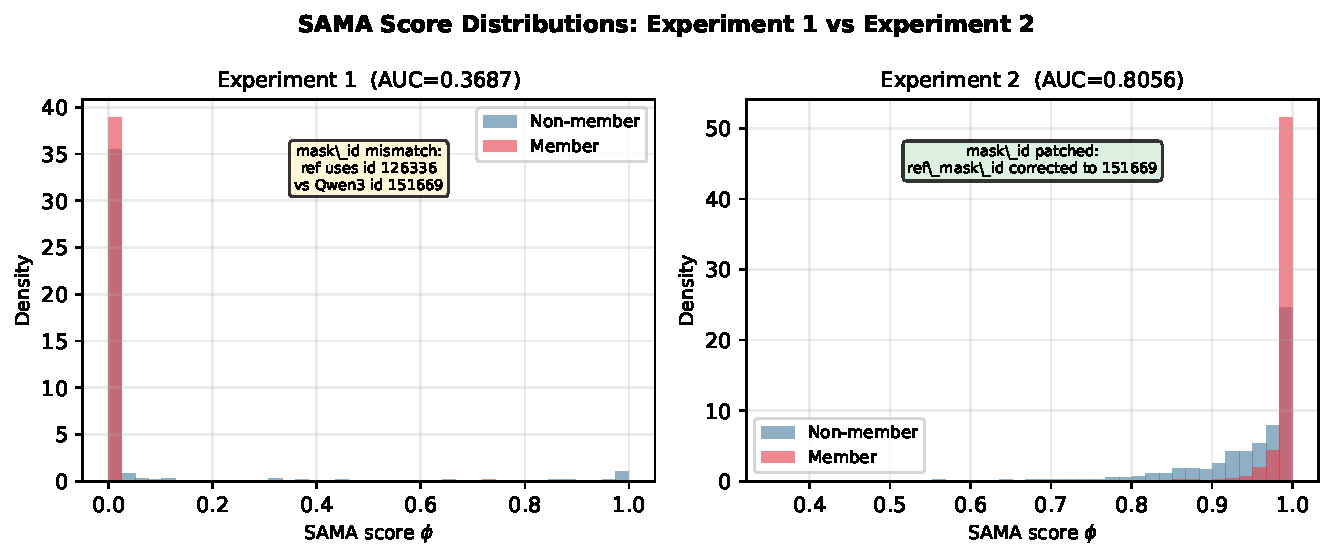
\includegraphics[width=\textwidth]{exp1_vs_exp2_sama.pdf}
    \column{0.45\textwidth}
    \textbf{SAMA achieves AUC = 0.806}, best scalar baseline.\\[8pt]
    But: \textbf{TPR@0.1\%FPR = 0.4\%}, near zero.\\[8pt]
    \textbf{Why?} $\phi(x)$ is one number.
    It can separate distributions in aggregate (AUC),
    but at the tails, where member and non-member scores overlap most -
    a scalar gives no way to discriminate further.
  \end{columns}
\end{frame}

% ── DT-MIA ───────────────────────────────────────────────────────────────────

\begin{frame}{DT-MIA: The Full Feature Vector}
  Instead of one scalar, we extract a \textbf{112-dimensional feature vector} from the diffusion trajectory:
  \vspace{6pt}
  \begin{tabular}{p{3.4cm} p{3.8cm} p{5.8cm}}
    \toprule
    \textbf{Signal} & \textbf{Formula} & \textbf{What it captures}\\
    \midrule
    ELBO trajectory
      & $\mathcal{L}(t_k) = -\log p_\theta(x_0\mid x_{t_k})$
      & How much the model fits $x_0$ at each noise level\\[4pt]
    Predictive entropy
      & $H(t_k) = -\sum_v p_\theta(v\mid x_{t_k})\log p_\theta(v\mid x_{t_k})$
      & Model confidence at each noise level; lower for members\\[4pt]
    Denoising consistency
      & $c(t_k) = \Pr[\hat x^{(1)} = \hat x^{(2)}]$
      & Stability of predictions under two random masking draws\\[4pt]
    Attention entropy
      & $H_{\mathrm{attn}}(t_k)$
      & Focus of attention: members have more concentrated patterns\\[4pt]
    Aggregates
      & variance, curvature, AUC-loss, \ldots
      & Shape of the trajectory, not just point values\\[4pt]
    Cross-model sim.
      & $\cos(\bar h_\theta, \bar h_{\theta_0})$
      & How much fine-tuning changed internal representations\\
    \bottomrule
  \end{tabular}
\end{frame}

\begin{frame}{Results: Benchmark}
  \begin{table}
    \small
    \setlength{\tabcolsep}{5pt}
    \begin{tabular}{llcccc}
      \toprule
      & \textbf{Method} & \textbf{AUC}
        & \textbf{TPR@0.1\%} & \textbf{TPR@1\%} & \textbf{TPR@10\%}\\
      \midrule
      \multirow{4}{*}{\rotatebox{90}{\tiny Baselines}}
        & Loss  & 0.699 & 4.0\%  &  9.9\% & 31.1\%\\
        & Zlib  & 0.715 & 4.7\%  & 10.8\% & 33.4\%\\
        & Ratio & 0.700 & 3.7\%  &  8.3\% & 31.2\%\\
        & SAMA  & 0.806 & 0.4\%  &  4.2\% & 42.1\%\\
      \midrule
      \multirow{2}{*}{\rotatebox{90}{\tiny Ours}}
        & \textbf{XGBoost} & \textbf{0.856} & \textbf{17.1\%} & \textbf{27.3\%} & \textbf{59.8\%}\\
        & MLP     & 0.854 &  5.1\% & 23.2\% & 58.8\%\\
      \bottomrule
    \end{tabular}
  \end{table}
\end{frame}

\begin{frame}{Results: ROC Curves}
  \begin{columns}
    \column{0.5\textwidth}
    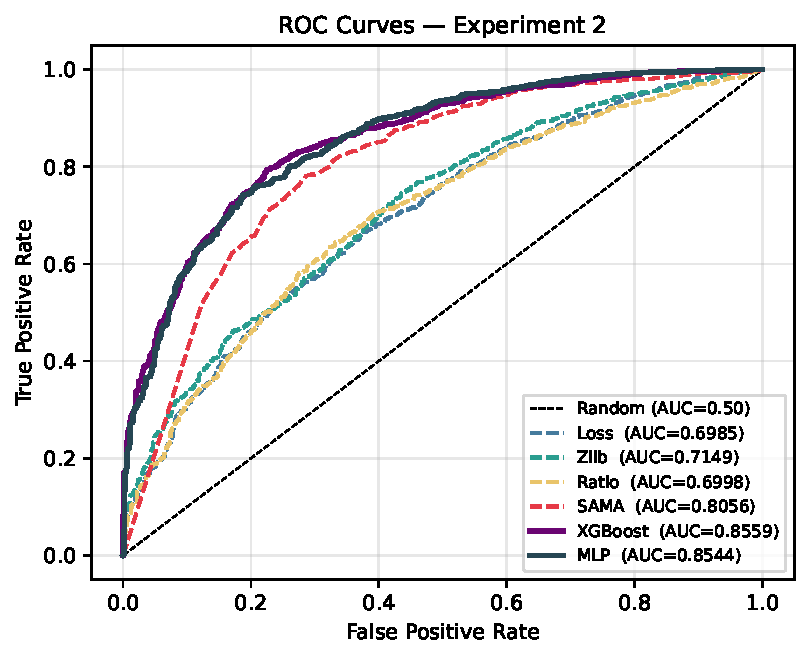
\includegraphics[width=\textwidth]{benchmark_roc.pdf}
    \column{0.5\textwidth}
    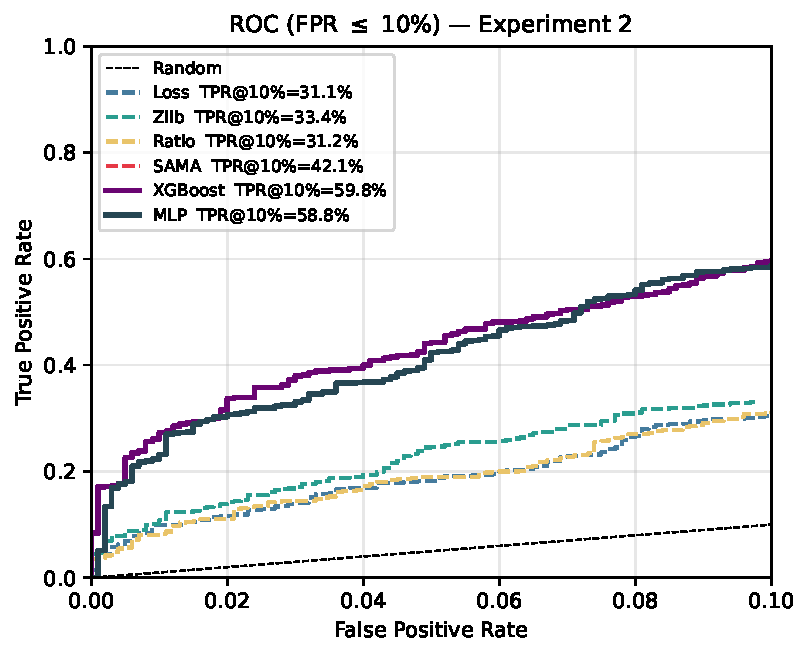
\includegraphics[width=\textwidth]{benchmark_roc_low_fpr.pdf}
  \end{columns}
  Left: full ROC. Right: zoomed to FPR $\leq 10\%$.
  Our classifiers dominate across the entire FPR range.
\end{frame}

\begin{frame}{Results: TPR Comparison}
  \begin{center}
    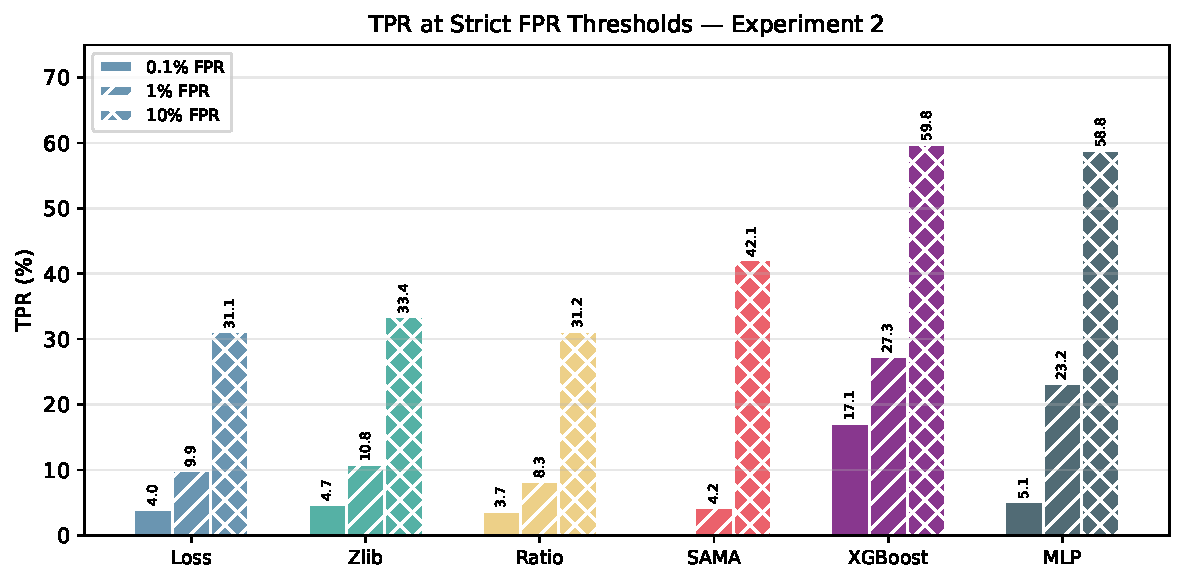
\includegraphics[width=0.85\textwidth]{tpr_all_methods.pdf}
  \end{center}
  Advantage is largest at 0.1\% FPR, the most privacy-relevant threshold.
\end{frame}

\begin{frame}{Feature Analysis}
  \begin{center}
    
\includegraphics[width=0.88\textwidth]{feature_heatmap.pdf}
  \end{center}
  Signal concentrates at \textbf{low noise levels} (small $t$, left side).
  Consistent with per-instance DP theory: leakage concentrates in the low-noise regime.
\end{frame}

\begin{frame}{The Key Number}
  At the practically relevant $0.1\%$ FPR:
  \begin{center}
    \begin{tabular}{lc}
      \toprule
      Method & TPR @ 0.1\% FPR\\ \midrule
      Loss / Zlib / Ratio & 3.7–4.7\%\\
      SAMA                & 0.4\%\\
      \textbf{DT-MIA (XGBoost)} & \textbf{17.1\%}\\
      \bottomrule
    \end{tabular}
  \end{center}
  \vspace{8pt}
  \textbf{40$\times$ more true positives than SAMA at the same false-positive budget.}\\[6pt]
  Scalar scores saturate at the tails.
  The trajectory shape carries independent information at every noise level.
\end{frame}

\begin{frame}{Future Directions}
  \begin{enumerate}
    \item \textbf{Full benchmark:} extend to all 9 MIMIR domains and LLaDA-8B
    \item \textbf{Per-instance DP auditing:} connect DT-MIA scores to theoretical $\varepsilon_i$-DP leakage
    \item \textbf{Trajectory shape:} curvature and variance of the loss curve as additional signals
    \item \textbf{Private fine-tuning:} exploit multiple masking realizations per sample for noise-multiplicity DP-SGD
  \end{enumerate}
\end{frame}

\begin{frame}{Summary}
  \begin{itemize}
    \item Diffusion models learn to reverse a noise process; DDPM does this for images with Gaussian noise
    \item The ELBO is the tractable objective, derived from MLE via Jensen's inequality and Markov structure
    \item For text, noise = masking; MDLM's objective is masked CE over all noise levels
    \item Most MIA baselines collapse the diffusion trajectory to a scalar and miss shape information
    \item DT-MIA reads the full 112-dimensional trajectory, achieving \textbf{40$\times$ improvement} at 0.1\% FPR
  \end{itemize}
  \vspace{14pt}
  \begin{center}
    \Large Thank you!\quad Questions?
  \end{center}
\end{frame}

\begin{frame}[allowframebreaks]{References}
  \bibliographystyle{plainnat}
  \bibliography{pres_refs}
\end{frame}

\end{document}
